\section{Radial velocity}

The first detection of an exoplanet was achieved by measuring the variation in the stellar radial velocity induced by the planet’s orbital motion, observed through the Doppler shift of the stellar spectrum.

\begin{figure}[]
\begin{center}
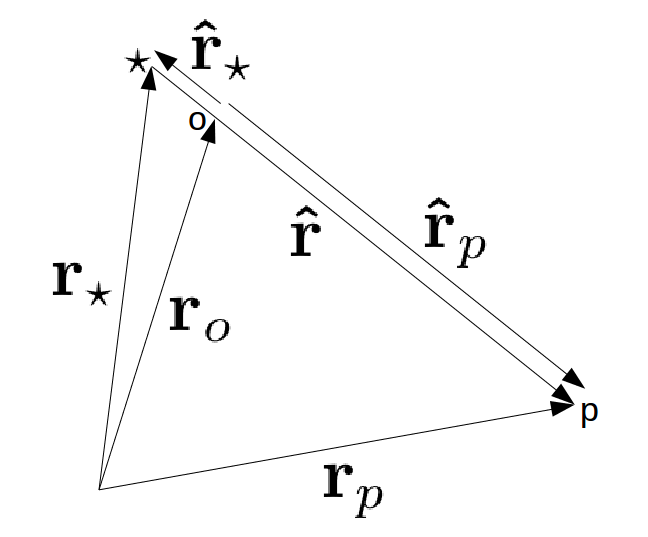
\includegraphics[bb=0 0 648 537,width=1.0\linewidth]{fig/rvector.png}
\end{center}
\caption{Definition of the barycenter $o$ and each vector.\label{fig:rvector}}
\end{figure}

We now consider the radial velocity variation of a star caused by an orbiting planet. In the two-body case, the observed stellar radial velocity corresponds to the motion of the vector measured from the system barycenter. As shown in Fig.~\ref{fig:rvector}, let the planet be denoted by $p$, the star by $\star$, and their barycenter by $o$. The stellar and planetary masses are $M_\star$ and $M_p$, and their positions are ${\bf r}_\star$ and ${\bf r}_p$, respectively. The barycenter ${\bf r}_o$ of this system is given by
\begin{eqnarray}
{\bf r}_o = \frac{M_\star {\bf r}_\star+ M_p {\bf r}_p}{M_\star + M_p}
\label{eq:rbary}
\end{eqnarray}
The positions relative to the barycenter are defined as ${\bf \hat{r}}_\star = {\bf r}_\star - {\bf r}_o$, ${\bf \hat{r}}_p = {\bf r}_p - {\bf r}_o$, and the vector from the star to the planet as ${\bf \hat{r}} = {\bf \hat{r}}_p - {\bf \hat{r}}_\star$. Then,
\begin{align}
\label{eq:barycentsp}
M_\star {\bf \hat{r}}_\star + M_p {\bf \hat{r}}_p &= M_\star {\bf \hat{r}}_\star + M_p ({\bf \hat{r}}_\star + {\bf \hat{r}} ) = 0 ,
\end{align}
which gives
\begin{eqnarray}
\label{eq:relpossp}
{\bf \hat{r}}_\star = - \frac{M_p}{M_\star + M_p} {\bf \hat{r}} .
\end{eqnarray}

The position vector of the star as seen by the observer can then be expressed using the barycenter position vector ${\bf r}_o$:
\begin{eqnarray}
{\bf r}_\star = {\bf r}_o + {\bf \hat{r}}_\star .
\end{eqnarray}
Since the star moves in the opposite direction to the planet, let us take the line of sight along the negative $Z$-axis and, in order to preserve the counterclockwise orientation, set $\Omega = \pi$. In this case, the stellar radial velocity is given by the negative of the inner product of the time derivative with the unit vector ${\bf e}_Z$ in the $Z$ direction,
\begin{eqnarray}
\label{eq:vrsatare}
v_r = V_\mathrm{sys} - \dot{\hat{\bf r}}_\star \cdot {\bf e}_Z ,
\end{eqnarray}
where $V_\mathrm{sys} \equiv - \dot{{\bf r}}_o \cdot {\bf e}_Z $ is the systemic velocity of the entire system. From Eq.~(\ref{eq:relpossp}),
\begin{eqnarray}
\label{eq:vrsatare2}
v_r = V_\mathrm{sys} + \frac{M_p}{M_\star + M_p} \dot{\hat{\bf r}} \cdot {\bf e}_Z .
\end{eqnarray}
Here, ${\bf \hat{r}}$ corresponds to ${\bf r}$ in the two-body problem in the previous section, so the same formalism can be applied directly. Thus, $\dot{\hat{\bf r}}_\star \cdot {\bf e}_Z$ corresponds to the time derivative of the $Z$ component in the three-dimensional coordinate system, $\dot{Z}$. Using Eq.~(\ref{eq:threed}),
\begin{eqnarray}
\label{eq:vrsatare3}
v_r &=& V_\mathrm{sys} + \frac{M_p}{M_\star + M_p} \dot{Z} ,
\end{eqnarray}
with
\begin{align}
\dot{Z} &= \frac{d}{d t} \left[ r \sin{i} \sin{(f + \omega)} \right] \nonumber \\
&= \dot{r} \sin{i} \sin{(f + \omega)} + r \dot{f} \sin{i} \cos{(f + \omega)} .
\end{align}

Using Eq.~(\ref{eq:dotr}), $r \dot{f} = h/r$, and the conic equation (\ref{eq:conic_kepler}), we obtain
\begin{align}
\label{eq:vrsatare4}
&v_r =V_\mathrm{sys} + \frac{M_p}{M_\star + M_p} \frac{h \sin{i}}{a (1-e^2)} [ e \sin{f} \sin{(f+\omega)} \nonumber \\
&+ e \cos{f} \cos{(f+\omega)} + \cos{(f+\omega)} ] \\
&=V_\mathrm{sys} + \frac{M_p}{M_\star + M_p} \frac{h \sin{i}}{a (1-e^2)} \left[ \cos{(f+\omega)} + e \cos{\omega} \right] \nonumber \\
\end{align}

\begin{itembox}{$\clubsuit$}
\footnotesize
\color{gray}
$\sin{f} \sin{(f+\omega)} + \cos{f} \cos{(f+\omega)} = \cos{(-f)} \cos{(f+\omega)} - \sin{(-f)} \sin{(f+\omega)} = \cos{(-f + f + \omega)} = \cos{\omega}$
\end{itembox}

Alternatively, writing out $h$ explicitly, we obtain
\begin{align}
\label{eq:vrsatarefinal}
v_r &= V_\mathrm{sys} + K_\star \left[ \cos{(f+\omega)} + e \cos{\omega} \right] \\
\label{eq:vrKrv}
K_\star &\equiv \frac{M_p \sin{i}}{\sqrt{1 - e^2}} \sqrt{\frac{G}{(M_p + M_\star) a}} ,
\end{align}
which represents the radial velocity curve of the two-body problem. The order of magnitude of the radial velocity variation is
\begin{align}
K_\star &\sim 30 \mathrm{m/s} , \frac{M_p \sin{i}}{M_J}\left(\frac{M_\star}{M_\odot} \right)^{-1/2} \left(\frac{a}{\mathrm{au}} \right)^{-1/2} \\
&= 130 \mathrm{m/s} , \frac{M_p \sin{i}}{M_\oplus}\left(\frac{M_\star}{M_\odot} \right)^{-1/2} \left(\frac{a}{0.05 \mathrm{au}} \right)^{-1/2} \mbox{(HJ)} \nonumber \\
&= 0.1 \mathrm{m/s} , \frac{M_p \sin{i}}{M_\oplus}\left(\frac{M_\star}{M_\odot} \right)^{-1/2} \left(\frac{a}{\mathrm{au}} \right)^{-1/2} \mbox{(Earth)} \nonumber
\end{align}
The Doppler shift corresponding to this radial velocity variation is
\begin{align}
\frac{\Delta \lambda}{\lambda} &\sim \frac{K_\star}{c} \nonumber \\
& = 10^{-7} \frac{M_p \sin{i}}{M_J} \left(\frac{M_\star}{M_\odot} \right)^{-1/2} \left(\frac{a}{\mathrm{au}} \right)^{-1/2} .
\end{align}

Since the spectral resolution of current high-dispersion spectrographs is $R \sim 10^5$, it is important to boost the signal-to-noise ratio using many molecular absorption lines (and photon counts). In practice, stabilizing wavelength calibration with iodine cells or frequency combs is also crucial.

\begin{itembox}{$\clubsuit$}
%\tiny
\footnotesize
\color{gray}
\begin{align}
    K_\star &\sim \frac{M_p \sin{i}}{M_\odot}\left(\frac{M_\star}{M_\odot} \right)^{-1/2}  \sqrt{ \frac{G M_\odot}{a} } \nonumber \\
    &= \frac{M_p \sin{i}}{M_\odot}\left(\frac{M_\star}{M_\odot} \right)^{-1/2} \sqrt{ \frac{2 G M_\odot}{c^2}\frac{1}{2a} } \, c \nonumber \\
    &= \frac{M_J}{M_\odot} \frac{M_p \sin{i}}{M_J} \left(\frac{M_\star}{M_\odot} \right)^{-1/2} \sqrt{ \frac{r_g}{2  \mathrm{au}} \frac{\mathrm{au}}{a} }\, c \nonumber \\
    &= 10^{-7} c \frac{M_p \sin{i}}{M_J}  \left(\frac{M_\star}{M_\odot} \right)^{-1/2} \left(\frac{a}{\mathrm{au}} \right)^{-1/2} \nonumber \\
    &= 30 \mathrm{m/s} \, \frac{M_p \sin{i}}{M_J}\left(\frac{M_\star}{M_\odot} \right)^{-1/2} \left(\frac{a}{\mathrm{au}} \right)^{-1/2} \nonumber
\end{align}
\end{itembox}


\subsection*{Radial velocity curve as a function of time}

In actual observations, measurements are obtained as functions of time, so we would like to express the solution in terms of time. From the time $t$ and the orbital period, the mean anomaly $M$ can be determined. The eccentric anomaly $E$ is then obtained by numerically solving Eq.~(\ref{eq:dee_sol_M}). Using these, Eq.~(\ref{eq:vrsatarefinal}) can be rewritten numerically as a function of time.

Thus, the physical quantities that can be derived from the radial velocity curve are, from Eq.~(\ref{eq:vrsatarefinal}), $V_\mathrm{sys}, K_\star, e, \omega$. In addition, the orbital period $P$ and a phase parameter (the time offset) related to $f$ can also be estimated. Figure~\ref{fig:rvsim} shows several radial velocity curves and the corresponding elliptical orbits. According to Kepler’s second law, one can see that the radial velocity curve changes rapidly when the body approaches periastron.

\begin{figure}[]
\begin{center}
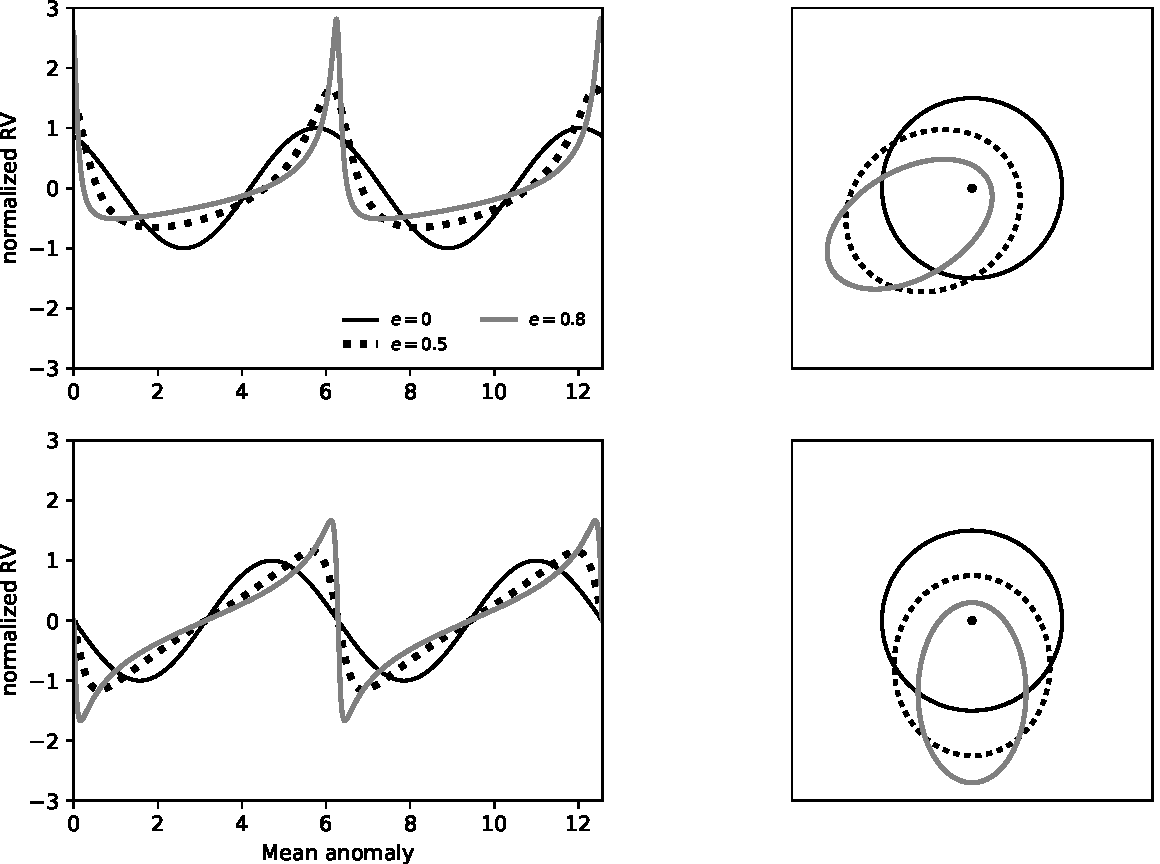
\includegraphics[width=\linewidth]{fig/rvsim.pdf}
\end{center}
\caption{Radial velocity curves (left) and corresponding orbits (right). The upper panels are for $\omega=\pi/6$, and the lower panels are for $\omega=\pi/2$. Line styles: black solid line for $e=0$, black dashed line for $e=0.5$, and gray solid line for $e=0.8$. The ellipses on the right correspond to orbits viewed from above when $i=\pi/2$. If the line of sight is taken from bottom to top, they correspond to the stellar orbit in the radial velocity curve, while if taken from top to bottom, they correspond to the planetary orbit. \label{fig:rvsim}}
\end{figure}

\begin{itembox}{Binary Mass Function$,^\dagger$}
%\tiny
\footnotesize
\color{gray}
Radial velocity analysis was originally developed for binary star systems before it was applied to star–planet systems. In this case, the approximation $M_p \ll M_\star$ does not hold. Rewriting Eq.~(\ref{eq:vrKrv}) with $\star \to 1$ and $p \to 2$, and using Kepler’s third law (\ref{eq:kep3}), we can separate the right-hand side into observable quantities and the left-hand side into physical parameters, giving
\begin{align}
\label{eq:bmfunc}
f \equiv \frac{M_2^3}{(M_1 + M_2)^2} \sin^3{i} = \frac{P K_1^3}{2 \pi G} (1 - e^2)^{3/2} .
\end{align}
Here, $f$ is a quantity that can be determined solely from the observed parameters of star 1’s radial velocity curve, $K_1$, $e$, and $P$, even in the general case of arbitrary mass ratios. This $f$ is called the binary mass function\index{Binary Mass Function@Binary Mass Function}.

Conversely, using a scaled form,
\begin{align}
\label{eq:semiamp2}
K_1 &= 29.8 , [\mathrm{km/s}] \frac{\sin{i}}{\sqrt{1 - e^2}} \left( \frac{M_2}{M_1 + M_2} \right) \nonumber \\
&\times \left( \frac{M_1 + M_2}{M_\odot} \right)^{1/3} \left( \frac{P}{1 \mathrm{yr}} \right)^{1/3} ,
\end{align}
is useful for estimating the detectability in the case of binary systems. The value 29.8 km/s corresponds to the Earth’s orbital velocity.
\end{itembox}


\section{Astrometry}

The radial velocity variation makes use of the $\dot{Z}$ component of the three-dimensional Keplerian motion. Since astrometry is the method of measuring the position of a star on the celestial sphere, it makes use of the ($X,Y$) components of the motion. After correcting for proper motion and parallax, the position of the star due to two-body motion can be expressed as an observable angle,
\begin{align}
{\boldsymbol{\theta}} = \frac{\hat{\rv}_\star}{d} = - \frac{M_p}{M_\star + M_p} \frac{\hat{\rv}}{d} ,
\end{align}
which is a two-dimensional projection, where $d$ is the distance between the observer and the star. From Eq.~(\ref{eq:threed}), we have
\begin{align}
\theta_x &= - \frac{M_p}{M_\star + M_p} \frac{X}{d} = - \frac{M_p}{M_\star + M_p} \frac{r}{d} \nonumber\\
&\times [\cos \bigl(f+\omega\bigr)\cos\Omega
- \sin \bigl(f+\omega\bigr)\cos i \, \sin\Omega] \\
\theta_y &= - \frac{M_p}{M_\star + M_p} \frac{Y}{d} =- \frac{M_p}{M_\star + M_p}\frac{r}{d} \nonumber\\
&\times [ \cos \bigl(f+\omega\bigr) \sin\Omega 
+ \sin \bigl(f+\omega\bigr)\cos i \,\cos\Omega] .
\end{align}

This solution is invariant under the transformation ($i \to \pi - i$, $f \to 2 \pi - f$, $\omega \to 2 \pi - \omega$), which means that astrometry alone cannot distinguish whether the planet is approaching or receding.